\chapter{Introduction}\label{chap:Intro}

\section{L'entreprise Obeo}
\kwobeo{} est une société de service et un éditeur de logiciels \cite{obeo}. Son expertise dans le domaine de l'ingénierie des modèles (démarche MDA), lui permet de proposer des solutions allant de la création à la refonte d'applications informatiques. 
 OB
\begin{figure}[htb]
  \centering
  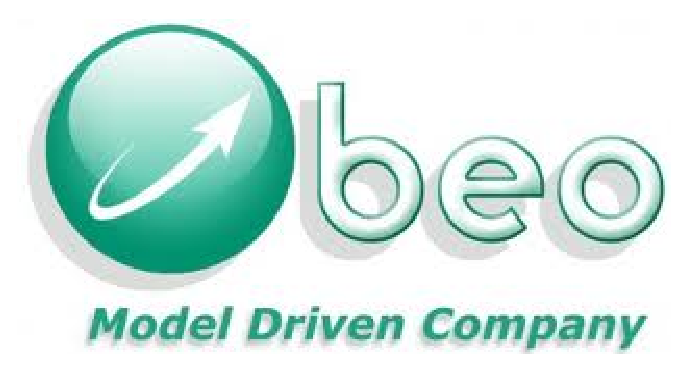
\includegraphics[scale=.4]{img/logoobeo.eps}
  \label{fig:obeo}
\end{figure}

Ces solutions proposées permettent notamment de diminuer les délais de projets et de diminuer les risques d'erreurs. Les amélioration des performances d'adaptation et d'agilité font aussi parties des objectifs des outils et méthode de la société \kwobeo{}.

La société \kwobeo{} est aussi un membre actif dans le domaine Open Source et est membre de la fondation Eclipse. Elle est à l'initiative du projet Acceleo, un générateur de code basé sur le framework EMF. 


\section{Acceleo et démarche M2T}
Acceleo est un projet Open Source de la fondation Eclipse dont \kwobeo{} est à l'origine (\cf{} \cite{acceleo}). À partir de modèles basé sur le framework EMF (\cf{} \cite{emf}), Acceleo permet de générer du code en mettant en œuvre l'approche Model driven architecture (MDA). Le générateur Acceleo est une implémentation de la norme de l'Object Management Group \cite{omg} pour les transformations de modèle vers texte (Model to Text : M2T).


%%  LocalWords:  Obeo MDA Acceleo
